The Low Level Dynamic~(LLD) semantics removes all the non-deterministic choices
in the previous dynamics and makes them deterministic. The new semantics will do
the following:

\begin{itemize}

   \item Match rules by priority order;

   \item Determine the set of linear facts needed to match either the body of
   the rule or the body of comprehensions without guessing;

   \item Apply as many comprehensions as the database allows.

   \item Apply as many aggregates as the database allows.

\end{itemize}

The complete set of inference rules for the semantics are presented in
Appendix~\ref{sec:lld}.

HLD had many different proof trees for a given triplet $\Gamma; \Delta; \Phi$
because HLD allows choices to be made during the inference rules. For instance,
in HLD any rule could be selected to be executed. In LLD there is only
one proof tree for a given $\Gamma; \Delta; \Phi$ since there is no
guessing involved. LLD semantics present a complete step by step
mechanism that is needed to correctly evaluate an LM program. For
instance, when LLD tries to apply a rule, it will check if there is
enough facts in the database and backtrack until a rule can be applied.

\begin{theorem}[Proof uniqueness]
In LLD, there is only one possible proof for a given $\Gamma; \Delta; \Phi$.
\end{theorem}
\begin{proof}

Inference rules of every judgment in LLD are disjunct, therefore only one
inference rule can be applied at any given point in the proof.

\end{proof}

LLD shares exactly the same inputs and outputs as HLD. The first difference
between the two systems starts when picking a rule to derive.  Instead of
guessing, LLD treats the list of rules as a stack and picks the first rule $R$
to execute (the rule with the highest priority). The remaining rules are stored
as a \emph{continuation}. If $R$ cannot be matched because there is not enough
facts in the database, we backtrack and use the rule continuation to pick the
next rule and so on, until one rule can be successfully applied.

\subsection{Continuation Frames}

The most interesting aspects introduced by LLD are the \emph{continuation frame}
and the \emph{continuation stack}. A continuation frame acts as a choice point
that is created during rule matching whenever we try to match a fact expression
against the database.  The frame considers all the facts relevant to the
expression given the current variable bindings and predicate, that may or not
fail during the remaining matching process.

The frame contains enough state to resume the matching process at the time of
its creation, therefore we can easily backtrack to the choice point and select
the next candidate fact from the database (judgment $\contlld$ or $\contclld$).
We keep the continuation frames in a continuation stack for backtracking
purposes. If a given fact fails, we update the top frame to try the next
candidate fact. If all candidates are exhausted, we pop the top frame and
continue with the next available frame.

By using this match mechanism, we determine which facts need to be used to match
a rule.  Our LM implementation works like LLD, by iterating over the available
facts at each choice point and then committing to the rule if the matching
process succeeds. However, while the implementation only attempts to match rules
with a very high change of success, LLD is more na\"{i}ve in this aspect because
it tries all rules in order.

\subsection{Structure of continuation frames}

We have two continuation frame types, depending on the type of the candidate
facts.

\subsubsection{Persistent continuation frame}

A \emph{persistent frame} has the form $[\Gamma'; \Delta; \Xi; \bang p; \Omega;
\Lambda; \Upsilon]$, where:

\begin{enumerate}

   \item[$\Gamma'$] remaining candidate facts;

   \item[$\Delta$] remaining multi-set of linear facts;

   \item[$\Xi$] multi-set of linear facts we have consumed to reach this point;

   \item[$\bang p$] current fact expression that originated this choice point;

   \item[$\Omega$] ordered list of remaining terms needed to match past this
   choice point;

   \item[$\Lambda$] multi-set of linear fact expressions that we have matched to
   reach this choice point. All the linear facts that match these terms are
   located in $\Xi$;

   \item[$\Upsilon$] multi-set of persistent fact expressions that we matched up
   to this point.

\end{enumerate}

\subsubsection{Linear continuation frame}

A \emph{linear frame} has the form $(\Delta; \Delta'; \Xi; p; \Omega; \Lambda;
\Upsilon)$, where:

\begin{enumerate}

   \item[$\Delta$] multi-set of linear facts that are not of type $p$ plus all
   the other $p$'s we have already tried, including the current $p$;

   \item[$\Delta'$] all the other $p$'s we haven't tried yet. It is a multi-set
   of linear facts;

   \item[$\Xi$] multi-set of linear facts we have consumed to reach this point;

   \item[$p$] current fact expression that originated this choice point;

   \item[$\Omega$] ordered list of remaining terms needed to match past this
   choice point;

   \item[$\Lambda$] multi-set of linear fact expressions that we have matched to
   reach this choice point. All the linear facts that match these terms are
   located in $\Xi$;

   \item[$\Upsilon$] multi-set of persistent fact expressions that we matched up
   to this point.

\end{enumerate}

\subsection{Step}

The starting inference rule of LLD is identical to the rule described
in~\ref{sec:step_hld} for HLD:

\[
\infer[\stepo]
{\begin{split}
\stepo [\Gamma_1, \dotsc, \Gamma_i, \dotsc, \Gamma_n] &; [\Delta_1, \dotsc,
   \Delta_i, \dotsc, \Delta_n];
   \Phi \\ \Longrightarrow& \\ [\Gamma_1, \Gamma'_1, \dotsc, \Gamma_i, \Gamma'_i,
   \dotsc,
   \Gamma_n, \Gamma'_n]; & [\Delta_1, \Delta'_1, \dotsc, (\Delta_i - \Xi'),
   \Delta'_i, \dotsc, \Delta_n, \Delta'_n]
\end{split}
}
{
   \doo \Gamma_i; \Delta_i; \Phi \rightarrow \Xi'; \Delta'_1, \dotsc, \Delta'_n;
   \Gamma'_1, \dotsc, \Gamma'_n
}
\]


\subsection{Application}

When starting a step, we pick the first rule $R_1$ and create a rule
continuation with the form $(\Phi, \Delta)$, where $\Phi$ is the stack of
remaining rules and $\Delta$ is the starting linear context. Context $\Gamma$
does not need to be saved because its facts are persistent.


\[
\trans{\dostate{\Delta}{R_1, \Phi}{\Gamma}{\Pi}}
{\appstate{\cdot}{\Delta}{\Phi}{\Pi}{\Gamma}{R}} \tag{select rule}
\]


\[
\trans{\dostate{\Delta}{\cdot}{\Gamma}{\Pi}}
   {\failstate{\Gamma}{\Delta}} \tag{fail}
\]


\[
   \trans{\appstate{\Psi}{\Delta}{\Phi}{\Pi}{\Gamma}{\forall_{x : \tau}. A}}
   {\appstate{\Psi, x : \_ : \tau}{\Delta}{\Phi}{\Pi}{\Gamma}{A}}
                                                             \tag{open rule}
\]


\[
   \trans{\appstate{\Psi}{\Delta}{\Phi}{\Pi}{\Gamma}{A \lolli B}}
   {\matstateb{A \lolli B}{(\Delta; \Phi)}{\cdot}{\Gamma}{\Delta}{A}{\cdot \rightarrow
   \one}{\Psi}} \tag{init
                                                            rule}
\]




\subsection{Match}\label{sec:lld_body_match}

The matchig judgment for LLD differs greatly from the same judgment in HLD. In
LLD, matching uses the continuation stack to try different combinations of facts
until a match is achieved. The matching judgment uses the form $\mo \Gamma;
\Delta; \Xi; \Omega; H; \lstack{C}; \lstack{R} \rightarrow \outsem$ where:

\begin{enumerate}

   \item[$\Delta$] multi-set of linear facts still available to complete the
   matching process;

   \item[$\Xi$] multi-set of linear facts consumed up to this point;

   \item[$\Omega$] ordered list of deconstructed head terms to match;

   \item[$H$] head of the rule;

   \item[$\lstack{C}$] ordered list of frames representing the continuation stack;

   \item[$\lstack{R}$] rule continuation to be used if the current rule fails;

   \item[$\outsem$] output contexts containing consumed facts and derived
   persistent and linear facts.

\end{enumerate}

Matching will attempt to use facts from $\Delta$ and $\Gamma$ to match the terms
of the body of the rule represented as $\Omega$. During this process
continuation frames are pushed into $\lstack{C}$.  If the matching process
fails, we use the continuation stack through the $\cont$judgment.

\subsubsection{Linear fact expression}

The first 4 inference rules are used when the head of $\Omega$ is a linear fact
expression $p$: (1) the continuation stack is empty; (2) the continuation is not
empty and a linear continuation frame is at the top; (3) the continuation stack
is not empty and a persistent continuation frame is at the top; and (4) we
cannot find any linear fact in the database that matches $p$. Note that in the
first 3 rules, we find $p_1$ and $\Delta''$ as facts from the database that
match $p$'s the hidden and partially initialized arguments.  Context $\Delta''$
is stored in the second argument of the new continuation frame but passes along
with $\Delta$ since they have not been consumed yet (just $p_1$).

Note that the proposition $p_1, \Delta'' \prec p$ indicates that facts
$\Delta'', p_1$ satisfy the constraints of $p$ while $\Delta \npreceq p$
indicates that no fact in $\Delta$ satisfies $p$.


\begin{multline}
\transx{\matstateb{A \lolli B}{\rulestk}{\lstack{C}}{\Gamma}{\Delta, p_1,
\Delta''}{p(\widehat{x}),
   \Omega}{\Delta' \rightarrow \Omega'}{\Psi}}
{\matstateb{A \lolli B}{\rulestk}{\lframe{\Delta,
p_1}{\Delta''}{p(\widehat{x})}{\Omega; \m{extend}(\Psi, \theta)}{\Delta'}{\Omega'}, \lstack{C}}{\Gamma}{\Delta,
   \Delta''}{\Omega}{\Delta', p_1 \rightarrow \Omega' \otimes
      p(\widehat{x}\theta)}{\m{extend}(\Psi, \theta)}} \\
   \;\;\; (p_1,
   \Delta'' \prec p(\widehat{x}) \;\;\; \Delta \npreceq p(\widehat{x}))
   \tag{match p ok}
\end{multline}

\begin{align}
   \trans{\matstate{A \lolli
   B}{\rulestk}{\lstack{C}}{\Gamma}{\Delta}{p(\widehat{x}),
   \Omega}{\Delta' \rightarrow \Omega'}}
{\contstate{A \lolli B}{\rulestk}{\lstack{C}}{\Gamma}} \;\;\; (\Delta \npreceq
p(\widehat{x})) \tag{match p fail}
\end{align}


\subsubsection{Persistent fact expressions}

The next 4 inference rules are used when the head of $\Omega$ contains a
persistent fact expression $\bang p$. They are identical to the previous 4 rules
but they deal with the persistent context $\Gamma$.

\begin{align}
\trans{\matstate{A \lolli B}{\rulestk}{\lstack{C}}{\Gamma}{\Delta}{\bang p,
   \Omega}{\Delta' \rightarrow \Omega'}}
{\matstate{A \lolli B}{\rulestk}{\pframe{\Gamma''}{\Delta}{\bang
   p}{\Omega}{\Delta'}{\Omega'}, \lstack{C}}{\Gamma, p_1,
      \Gamma''}{\Delta}{\Omega}{\Delta' \rightarrow \Omega' \otimes \bang p}}
      \;\;\; (\bang p_1, \Gamma'' \prec \bang p) \tag{match \bang p ok}
\end{align}

\begin{align}
\trans{\matstate{A \lolli B}{\rulestk}{\lstack{C}}{\Gamma}{\Delta}{\bang p,
   \Omega}{\Delta' \rightarrow \Omega'}}
{\contstate{A \lolli B}{\rulestk}{\lstack{C}}{\Gamma}} \;\;\; (\Gamma \npreceq
      \bang p) \tag{match \bang p fail}
\end{align}


\subsubsection{Other expressions}

Finally, we have the inference rule $\mo \otimes$ that deconstructs body terms
with $\otimes$ and the $\mo \m{end}$ rule that terminates the matching process
and initiates the derivation of head terms because $\Omega$ is empty.


\begin{align}
\trans{\matstate{A \lolli B}{\rulestk}{\lstack{C}}{\Gamma}{\Delta}{\one,
   \Omega}{\Delta' \rightarrow \Omega'}}
{\matstate{A \lolli B}{\rulestk}{\lstack{C}}{\Gamma}{\Delta}{\Omega}{\Delta'
   \rightarrow \Omega'}} \tag{match $\one$}
\end{align}

\begin{align}
\trans{\matstate{A \lolli B}{\rulestk}{\lstack{C}}{\Gamma}{\Delta}{X \otimes Y,
   \Omega}{\Delta' \rightarrow \Omega'}}
{\matstate{A \lolli B}{\rulestk}{\lstack{C}}{\Gamma}{\Delta}{X, Y,
   \Omega}{\Delta' \rightarrow \Omega'}} \tag{match $\otimes$}
\end{align}

\begin{align}
\trans{\matstate{A \lolli
   B}{\rulestk}{\lstack{C}}{\Gamma}{\Delta}{\cdot}{\Delta' \rightarrow \Omega'}}
{
   \derstatex{\Gamma}{\Delta}{\Delta'}{\cdot}{\cdot}{B}
} \tag{match end}
\end{align}


\subsection{Continuation}\label{sec:lld_match_cont}

If the matching process fails, we pick the top continuation frame from the stack
$\lstack{C}$ and restore the matching process using another candidate fact. The judgment
\mbox{$\cont \lstack{C}; H; \lstack{R}; \Gamma \rightarrow \outsem$} specifies the
backtracking process where the meaning of each argument is as follows:

\begin{enumerate}
   \item[$\lstack{C}$] continuation stack;
   \item[$H$] head of the current rule being executed;

   \item[$\lstack{R}$] next available rules if the current rule does not match.

\end{enumerate}

\subsubsection{Linear continuation frames}

The next two inference rules handle linear continuation frames on the top of the
continuation stack. The first rule selects the next candidate fact $p_1$ from the
second argument of the linear frame and updates the frame. Otherwise, if we have
no more candidate facts, we pop the continuation frame and use $\cont$again with
the remaining continuation stack.

\begin{align}
\trans{\contstate{A \lolli B}{\rulestk}{\lframe{\Delta}{p_2,
   \Delta''}{p}{\Omega}{\Delta'}{\Omega'}, \lstack{C}}{\Gamma}}
{
   \matstate{A \lolli B}{\rulestk}{\lframe{\Delta,
      p_2}{\Delta''}{p}{\Omega}{\Delta'}{\Omega'},
   \lstack{C}}{\Gamma}{\Delta}{\Omega}{\Delta', p_2 \rightarrow \Omega' \otimes p}}
   \tag{next p}
\end{align}

\begin{align}
\trans{\contstate{A \lolli
   B}{\rulestk}{\lframe{\Delta}{\cdot}{p}{\Omega}{\Delta'}{\Omega'},
      \lstack{C}}{\Gamma}}
{
   \contstate{A \lolli B}{\rulestk}{\lstack{C}}{\Gamma}} \tag{next frame}
\end{align}


\subsubsection{Persistent continuation frames}

We also have the same two kinds of inference rules for persistent continuation
frames.

\[
\infer[\cont \bang p~\m{next}]
{\cont [p_1, \Gamma'; \Delta; \bang p, \Omega; \Xi; \Lambda; \Upsilon], C; H; R; \Gamma \rightarrow \Xi'; \Delta'; \Gamma'}
{\mo \Gamma; \Delta; \Xi; \Omega; H; [\Gamma'; \Delta; \bang p, \Omega; \Xi; \Lambda; \Upsilon], C; R \rightarrow \Xi'; \Delta'; \Gamma'}
\]

\[
\infer[\cont \bang p~\m{no~more}]
{\cont [\cdot; \Delta; \bang p, \Omega; \Xi; \Lambda; \Upsilon], C; H; R; \Gamma \rightarrow \Xi'; \Delta'; \Gamma'}
{\cont C; H; R; \Gamma \rightarrow \Xi'; \Delta'; \Gamma'}
\]


\subsubsection{Empty continuation stack}

Finally, if the continuation stack is empty, we simply force execution to try
the next inference rule in $\Phi$.

\begin{align}
\trans{\contstate{A \lolli B}{(\Delta; \Phi)}{\cdot}{\Gamma}}
   {\dostate{\Delta}{\Phi}{\Gamma}{\Pi}} \tag{rule fail}
\end{align}


\subsection{Derivation}

Once the list of terms $\Omega$ in the $\mo$judgment is exhausted (rule $\mo
\m{end}$), we derive the head of rule.  The derivation judgment is
specified as $\done \Gamma; \Delta; \Xi; \Gamma_1; \Delta_1; \Omega \rightarrow
\outsem$, where:

\begin{enumerate}

   \item[$\Delta$] multi-set of linear facts we started with minus the linear
   facts consumed $\Xi$ during the matching of the body of the rule;

   \item[$\Xi$] multi-set of linear facts consumed during the matching of the
   body of the rule;

   \item[$\Gamma_1$] set of persistent facts derived up to this point in the
   derivation;

   \item[$\Delta_1$] multi-set of linear facts derived up to this point in the
   derivation;

   \item[$\Omega$] remaining terms to derive as an ordered list. We start with
   $B$ if the original rule is $A \lolli B$.

\end{enumerate}

\subsubsection{Fact templates}

When deriving either $p$ or $\bang p$ we have the following two inference rules:

\[
\infer[\done p]
{\done \Gamma ; \Delta; \Xi; \Gamma_1 ; \Delta_1; p, \Omega \rightarrow \outsem}
{\done \Gamma ; \Delta; \Xi; \Gamma_1 ; p, \Delta_1; \Omega \rightarrow \outsem}
\tab
\infer[\done \bang p]
{\done \Gamma ; \Delta ; \Xi; \Gamma_1 ; \Delta_1; \bang p, \Omega \rightarrow
   \outsem}
{\done \Gamma ; \Delta ; \Xi; \Gamma_1, p; \Delta_1; \Omega \rightarrow \outsem}
\]


\subsubsection{Deconstruct head}

The following two inference rules deconstruct the head list $\Omega$ from terms
created using either $1$ or $\otimes$.

\[
\infer[\done 1]
{\done \Gamma; \Delta; \Xi; \Gamma_1 ; \Delta_1; 1, \Omega \rightarrow \outsem}
{\done \Gamma; \Delta; \Xi; \Gamma_1 ; \Delta_1; \Omega \rightarrow \outsem}
\tab
\infer[\done \otimes]
{\done \Gamma ; \Delta; \Xi; \Gamma_1; \Delta_1; A \otimes B, \Omega \rightarrow
   \outsem}
{\done \Gamma ; \Delta; \Xi; \Gamma_1; \Delta_1; A, B, \Omega \rightarrow
   \outsem}
\]


\subsubsection{Comprehensions}

The inference rule $\done \m{comp}$ deals with comprehensions. We use the same
term \mbox{$AB = \compsz{A}{B}$} for comprehensions as before.  Judgment $\mc{AB}$initiates the
matching process of the body $A$ of the comprehension (explained in the next
section).

{\footnotesize
\[
\infer[\done \m{comp}]
{\done \Gamma; \Delta ; \Xi; \Gamma_1; \Delta_1; \compsz{A}{B}, \Omega \rightarrow \Xi';\Delta';\Gamma'}
{\mc \Gamma; \Delta; \Xi; \Gamma_1; \Delta_1; \cdot; A ; \cdot; \cdot;
   \compsz{A}{B}; \Omega; \Delta \rightarrow \Xi';\Delta';\Gamma'}
\]
}


\subsubsection{Aggregates}

The inference rule $\done \m{agg}$ deals with aggregates. We use the same term
\mbox{$\aggsz{A}{B}{C}$} for aggregates as before. Judgment
$\ma{\aggsz{A}{B}{C}}$initiates the matching process of the body $A$ of the
aggregate (explained in the next section).

\[
\infer[\done \m{agg}]
{\done \Gamma; \Delta ; \Xi; \Gamma_1; \Delta_1; \aggsz{A}{B}{C}, \Omega
   \rightarrow \outsem}
{\ma \Gamma; \Delta; \Xi; \Gamma_1; \Delta_1; \cdot; A ; \cdot; \cdot;
   \aggsz{A}{B}{C}; \Omega; \Delta; \cdot \rightarrow \outsem}
\]


\subsubsection{Successful rule}

Finally, if the ordered list $\Omega$ is exhausted, then the whole execution
process is done.  Note how the output arguments match the input arguments of the
$\done$judgment.

\begin{align}
\trans{\derstatex{\Gamma}{\Delta}{\Xi}{\Gamma_1}{\Delta_1}{\cdot}}
{\finalstate{\Xi}{\Gamma_1}{\Delta_1}} \tag{rule finished}
\end{align}


\subsection{Comprehensions}
The most intricate part of the derivation process is processing comprehensions
and aggregates. For both of them, we need to perform as many derivations as the
database allows, therefore we need to deterministically check the contents of
the database until no more derivations are possible.  The matching process is
then similar to the process used for matching the rule's LHS presented in
Section~\ref{sec:lld_body_match}, however we use two continuation stacks,
$\lstack{C}$ and $\lstack{P}$. In $\lstack{P}$, we put all the initial
persistent frames and in $\lstack{C}$ we put the first linear frame and then
everything else.

In order to reuse the stacks $\lstack{C}$ and $\lstack{P}$, we need to update them by removing all
the frames in $\lstack{C}$ pushed after the first linear continuation frame.  If we tried
to use those frames, we would assumed that the linear facts used by the other
frames were still in the database, but that is not true because they have been
consumed during the first application of the comprehension.  For example, if the
LHS is $\bang \mathtt{a(X)} \otimes \mathtt{b(X)} \otimes \mathtt{c(X)}$ and
the continuation stack has three frames (one per fact), we cannot backtrack to
the frame of $\mathtt{c(X)}$ because, at that point, the matching process was
assuming that the previous \texttt{b(X)} linear fact was still available.
Moreover, we also need to remove the consumed linear facts from the frames of
\texttt{b(X)} and $\bang$\texttt{a(X)} in order to make the stack fully
consistent with the new database. We will see later on how to do that.

The match judgment $\mc{AB} \Gamma; \Delta; \Xi_N; \Gamma_{N1}; \Delta_{N1};
\Xi; \Omega; \lstack{C}; \lstack{P}; \Omega_N; \Delta_N \rightarrow \outsem$ is
as follows:

\begin{enumerate}

   \item[$\Delta$] multi-set of linear facts remaining up to this point in the
   matching process;

   \item[$\Xi_N$] multi-set of linear facts used during the matching process of
   the rule's LHS and all the previous comprehensions;


   \item[$\Gamma_{N1}$] set of persistent facts derived up to this point in the
      rule's RHS;

   \item[$\Delta_{N1}$] multi-set of linear facts derived up to this point in
   the rule's RHS;

   \item[$\Xi$] multi-set of linear facts consumed up to this point;

   \item[$\Omega$] ordered list of terms that need to be matched for the
   comprehension to be applied;

   \item[$\lstack{C}$] continuation stack that contains both linear and
   persistent frames. The first frame must be linear;

   \item[$\lstack{P}$] initial part of the continuation stack with only persistent
   frames;


   \item[$\Omega_N$] ordered list of remaining terms of the rule's RHS to be
      derived;

   \item[$\Delta_N$] multi-set of linear facts that were still available after
   matching the rule's LHS and all the previous comprehensions. Note that
   $\Delta, \Xi = \Delta_N$.

\end{enumerate}

\subsubsection{Linear fact expressions}

The following five inference rules deal with the case when there is a linear
fact expression in the comprehension's LHS.


\[
\infer[\mc{AB} p~\m{first}]
{\mc{AB} \Gamma; \Delta, p_1, \Delta''; \Xi_N; \Gamma_{N1}; \Delta_{N1}; \cdot; p,
   \Omega; \cdot; \cdot; \Omega_N; \Delta_N \rightarrow \outsem}
{
   \begin{gathered}
      p_1, \Delta'' \prec p \\
      \mc{AB} \Gamma; \Delta, \Delta''; \Xi_N; \Gamma_{N1};
      \Delta_{N1}; \Xi, p_1; \Omega; (\Delta, p_1; \Delta''; \cdot; p; \Omega;
            \cdot; \cdot); \cdot; \Omega_N; \Delta_N \rightarrow \outsem
   \end{gathered}}
\]

\[
\infer[\mc{AB} p~\m{on}~q]
{\mc{AB} \Gamma; \Delta, p_1, \Delta''; \Xi_N; \Gamma_{N1}; \Delta_{N1}; \Xi; p,
   \Omega; f, \lstack{C}; \lstack{P}; \Omega_N; \Delta_N \rightarrow \outsem}
{
   \begin{gathered}
      p_1, \Delta'' \prec p \\
      f = (\Delta_{old}; \Delta'_{old}; \Xi_{old}; q; \Omega_{old}; \Lambda; \Upsilon) \\
      f' = (\Delta, p_1; \Delta''; \Xi; p; \Omega; q, \Lambda; \Upsilon) \\
      \mc{AB} \Gamma; \Delta, \Delta''; \Xi_N; \Gamma_{N1}; \Delta_{N1}; \Xi, p_1; \Omega;
      f', f, \lstack{C}; \lstack{P}; \Omega_N; \Delta_N \rightarrow \outsem
   \end{gathered}
}
\]


\[
\infer[\mc{AB} p~\m{on}~\bang q~\lstack{C}]
{\mc{AB} \Gamma; \Delta, p_1, \Delta''; \Xi_N; \Gamma_{N1}; \Delta_{N1}; \Xi; p,
   \Omega; f, \lstack{C}; \lstack{P}; \Omega_N; \Delta_N \rightarrow \outsem}
{
   \begin{gathered}
      p_1, \Delta'' \prec p \\
      f = [\Gamma_{old}; \Delta_{old}; \Xi_{old}; q; \Omega_{old}; \Lambda; \Upsilon] \\
      f' = (\Delta, p_1; \Delta''; \Xi; p; \Omega; \Lambda; q, \Upsilon) \\
      \mc{AB} \Gamma; \Delta, \Delta''; \Xi_N; \Gamma_{N1}; \Delta_{N1}; \Xi,
      p_1; \Omega; f', f, \lstack{C}; \lstack{P}; \Omega_N; \Delta_N \rightarrow \outsem
   \end{gathered}
}
\]


\[
\infer[\mc{AB} p~\m{on}~\bang q~\lstack{P}]
{\mc{AB} \Gamma; \Delta, p_1, \Delta''; \Xi_N; \Gamma_{N1}; \Delta_{N1}; \cdot; p,
   \Omega; \cdot; f, \lstack{P}; \Omega_N; \Delta_N \rightarrow \outsem}
{
   \begin{gathered}
      p_1, \Delta'' \prec p \\
      f = [\Gamma_{old}; \Delta_N; \cdot; q; \Omega_{old}; \cdot; \Upsilon]\\
      \Delta_N = \Delta, p_1, \Delta'' \\
      f' = (\Delta, p_1; \Delta''; \cdot; p; \Omega; \cdot; q, \Upsilon) \\
      \mc{AB} \Gamma; \Delta, \Delta''; \Xi_N; \Gamma_{N1}; \Delta_{N1}; p_1; \Omega;
         f'; f, \lstack{P};
         \Omega_N; \Delta_N \rightarrow \outsem
   \end{gathered}
}
\]


\[
\infer[\mc{AB} p~\m{fail}]
{\mc{AB} \Gamma; \Delta; \Xi_N; \Gamma_{N1}; \Delta_{N1}; \Xi; p, \Omega;
   \lstack{C}; \lstack{P}; \Omega_N; \Delta_N \rightarrow \outsem}
{\Delta \npreceq p & \contc \Gamma; \Delta_N; \Xi_N; \Gamma_{N1}; \Delta_{N1};
   \lstack{C}; \lstack{P}; \Omega_N \rightarrow \outsem}
\]


\subsubsection{Persistent fact expressions}

The inference rules for matching persistent fact expressions are similar to the
previous ones.


\[
\infer[\mc{AB} \bang p~\m{first}]
{\mc{AB} \Gamma, p_1, \Gamma''; \Delta_N; \Xi_N; \Gamma_{N1}; \Delta_{N1};
   \cdot; \bang p, \Omega; \cdot; \cdot; \Omega_N; \Delta_N \rightarrow \outsem}
{\begin{gathered}
   p_1, \Gamma'' \prec \bang p \\
   f = [\Gamma''; \Delta_N; \cdot; \bang p; \cdot; \Omega; \cdot; \cdot] \\
   \mc{AB} \Gamma, p_1, \Gamma''; \Delta_N; \Xi_N; \Gamma_{N1}; \Delta_{N1};
   \cdot; \Omega; \cdot; f;
   \Omega_N; \Delta_N \rightarrow \outsem
\end{gathered}
}
\]

\[
\infer[\mc{AB} \bang p~\m{on}~\bang q~\lstack{P}]
{\mc{AB} \Gamma, p_1, \Gamma''; \Delta_N; \Xi_N; \Gamma_{N1}; \Delta_{N1};
   \cdot; \bang p, \Omega; \cdot; f, \lstack{P}; \Omega_N; \Delta_N \rightarrow \outsem}
{
   \begin{gathered}
      p_1, \Gamma'' \prec \bang p \\
      f = [\Gamma_{old}; \Delta_N; \cdot; \bang q; \Omega_{old}; \cdot; \Upsilon] \\
      f' = [\Gamma''; \Delta_N; \cdot; \bang p; \cdot; \Omega; \cdot; q,
      \Upsilon] \\
      \mc{AB} \Gamma, p_1, \Gamma''; \Delta_N; \Xi_N; \Gamma_{N1}; \Delta_{N1};
      \cdot; \Omega; f', f, \lstack{P}; \Omega_N; \Delta_N \rightarrow \outsem
   \end{gathered}}
\]


\[
\infer[\mc{AB} \bang p~\m{on}~\bang q~\lstack{C}]
{\mc{AB} \Gamma, p_1, \Gamma''; \Delta; \Xi_N; \Gamma_{N1}; \Delta_{N1}; \Xi;
   \bang p, \Omega; f, \lstack{C}; \lstack{P}; \Omega_N; \Delta_N \rightarrow \outsem}
{
   \begin{gathered}
      p_1, \Gamma'' \prec \bang p \\
      f = [\Gamma_{old}; \Delta_{old}; \Xi_{old}; \bang q; \Omega_{old};
      \Lambda; \Upsilon] \\
      f' = [\Gamma''; \Delta; \Xi; \bang p; \cdot; \Omega; \Lambda; q, \Upsilon] \\
      \mc{AB} \Gamma,
      p_1, \Gamma''; \Delta; \Xi_N; \Gamma_{N1}; \Delta_{N1}; \Xi; \Omega; f', f,
      \lstack{C}; \lstack{P}; \Omega_N; \Delta_N \rightarrow \outsem
   \end{gathered}
}
\]


\[
\infer[\mc{AB} \bang p~\m{on}~q~\lstack{C}]
{\mc{AB} \Gamma, p_1, \Gamma''; \Delta; \Xi_N; \Gamma_{N1}; \Delta_{N1}; \Xi;
   \bang p, \Omega; f, \lstack{C}; \lstack{P}; \Omega_N; \Delta_N \rightarrow \outsem}
{
   \begin{gathered}
      p_1, \Gamma'' \prec \bang p \\
      f = (\Delta_{old}; \Delta'_{old}; \Xi_{old}; q; \Omega_{old}; \Lambda; \Upsilon) \\
      f' = [\Gamma''; \Delta; \Xi; \bang p; \cdot; \Omega; \Lambda, q; \Upsilon] \\
      \mc{AB} \Gamma, p_1, \Gamma''; \Delta; \Xi_N; \Gamma_{N1}; \Delta_{N1}; \Xi; \Omega;
      f', f, \lstack{C}; \lstack{P}; \Omega_N; \Delta_N \rightarrow \outsem
   \end{gathered}
}
\]

\[
\infer[\mc{AB} \bang p~\m{fail}]
{\mc \Gamma; \Delta; \Xi_N; \Gamma_{N1}; \Delta_{N1}; \Xi; \bang p, \Omega;
   \lstack{C}; \lstack{P}; \Omega_N; \Delta_N \rightarrow \outsem}
{\Gamma \npreceq \bang p & \contc{AB} \Gamma; \Delta_N; \Xi_N; \Gamma_{N1};
   \Delta_{N1}; \lstack{C}; \lstack{P}; \Omega_N \rightarrow \outsem}
\]


\subsubsection{LHS Deconstruction}

The inference rules for deconstructing the comprehension's LHS, including the
connectives $\otimes$ and $\one$, are shown next.


\[
\infer[\mc \otimes]
{\mc \Delta; \Xi_N; \Delta_{N1}; \Xi; X \otimes Y, \Omega; C; P; AB; \Omega_N; \Delta_N \rightarrow \Xi'; \Delta'}
{\mc \Delta; \Xi_N; \Delta_{N1}; \Xi; X, Y, \Omega; C; P; AB; \Omega_N; \Delta_N \rightarrow \Xi'; \Delta'}
\]


\subsubsection{Successful match}

Finally, when there is no more terms to match, we initiate the process of the
updating the continuation stack with $\fix{AB}$ followed by deriving the
comprehension's RHS.

\[
\infer[\mc{AB} \m{end}]
{\mc{AB} \Gamma; \Delta; \Xi_N; \Gamma_{N1}; \Delta_{N1}; \Xi; \cdot; \lstack{C};
   \lstack{P}; \Omega_N; \Delta_N \rightarrow \outsem}
{\fix{AB} \Gamma; \Delta; \Xi_N; \Gamma_{N1}; \Delta_{N1}; \Xi; \lstack{C}; \lstack{P}; \Omega_N; \Delta_N
   \rightarrow \outsem}
\]


\subsubsection{Continuation stack update}

As we said before, to update the continuation stacks, we need remove to all the
frames except the first linear frame and remove the consumed linear facts from
the remaining frames so that they are still valid for the next application of
the comprehension.  The judgment that updates the stack has the form $\fix{AB}
\Gamma; \Delta; \Xi_N; \Gamma_{N1}; \Delta_{N1}; \Xi; \lstack{C}; \lstack{P}; \Omega_N; \Delta_N
\rightarrow \outsem$, where:

\begin{enumerate}
   \item[$\Delta$] multi-set of linear facts remaining after matching the last
   comprehension;

   \item[$\Xi_N$] multi-set of linear facts used during the matching process of
      the rule's LHS and all the previous comprehensions;

   \item[$\Gamma_{N1}$] set of persistent facts derived by the rule's RHS and
      all the previous comprehensions;

   \item[$\Delta_{N1}$] multi-set of linear facts derived by the rule's RHS and
      all the previous comprehensions;

   \item[$\Xi$] multi-set of linear facts consumed by the previous application
   of the comprehension;
   \item[$\lstack{C}, \lstack{P}$] continuation stacks for the comprehension;

   \item[$\Omega_N$] ordered list of remaining terms of the rule's RHS to be
      derived;

   \item[$\Delta_N$] multi-set of linear facts that were still available after
   matching the rule's LHS and all the previous comprehensions.

\end{enumerate}

\subsubsection{Remove linear continuation frames}

To remove all linear continuation frames except the first one, we simply go
through all the frames in the stack $\lstack{C}$ with $\fix{AB} \m{more}$
until only one frame remains. This frame is then updated using $\fix{AB} \m{end~linear}$ by removing the linear facts $\Xi$ consumed
during the last application of the comprehension.

\[
\infer[\fix{\compsz{A}{B}} \m{end~linear}]
{\fix{\compsz{A}{B}} \Gamma; \Delta; \Xi_N; \Gamma_{N1}; \Delta_{N1}; \Xi; f; \lstack{P};  \Omega_N; \Delta_N \rightarrow \outsem}
{
   \begin{gathered}
      \strans \Xi; \lstack{P}; \lstack{P'} \\
      f = (\Delta_x; \Delta''; \cdot; p; \Omega; \cdot; \Upsilon) \\
      f' = (\Delta_x - \Xi; \Delta'' - \Xi; \cdot; p; \Omega; \cdot;
            \Upsilon) \\
      \dc{\compsz{A}{B}} \Gamma; \Delta; \Xi_N, \Xi; \Gamma_{N1};
      \Delta_{N1}; B; f' ; \lstack{P'} ; \Omega_N \rightarrow \outsem
   \end{gathered}
}
\]

\[
\infer[\fix{AB} \m{more}]
{\fix{AB} \Gamma; \Delta; \Xi_N; \Gamma_{N1}; \Delta_{N1}; \Xi; \_, f, \lstack{C};
   \lstack{P}; \Omega_N;
   \Delta_N \rightarrow \outsem}
{\fix{AB} \Gamma; \Delta; \Xi_N; \Gamma_{N1}; \Delta_{N1}; \Xi; f, \lstack{C};
   \lstack{P}; \Omega_N;
   \Delta_N \rightarrow \outsem}
\]

\[
\infer[\fix{\compsz{A}{B}} \m{end~empty}]
{\fix{\compsz{A}{B}} \Gamma; \Delta; \Xi_N; \Gamma_{N1}; \Delta_{N1}; \Xi; \cdot;
   \lstack{P}; \Omega_N; \Delta_N \rightarrow \outsem}
{\begin{gathered}
   \strans \Xi; \lstack{P}; \lstack{P'} \\
   \dc{\compsz{A}{B}} \Gamma; \Delta ; \Xi_N, \Xi; \Gamma_{N1};
      \Delta_{N1}; B; \cdot ; \lstack{P'} ; \Omega_N \rightarrow \outsem
 \end{gathered}
}
\]


\subsubsection{Transform persistent continuation frames}

Finally, we also need to subtract the consumed facts in $\Xi$ from the second
argument of every persistent continuation frame.  We have an auxiliary judgment
$\strans \Xi; \lstack{P}; \lstack{P'}$ where $\Xi$ is the multi-set of consumed
linear facts, $\lstack{P}$ is the persistent continuation stack and
$\lstack{P'}$ is the stack $\lstack{P}$ after the update.

\[
\infer[\strans]
{\strans \Xi; [\Gamma'; \Delta_N; \cdot; \bang p; \Omega; \cdot; \Upsilon], P; [\Gamma'; \Delta_N - \Xi; \cdot; \bang p, \Omega; \cdot; \Upsilon], P'}
{\strans \Xi; P; P'}
\]

\[
\infer[\strans \m{end}]
{\strans \Xi; \cdot; \cdot}
{\strans \Xi; \cdot; \cdot}
\]


\subsubsection{Comprehension continuation}

If the comprehension match fails, we need to backtrack to the previous frame and
restore the matching process at that point. The judgment used to backtrack is
similar to the one presented in Section~\ref{sec:lld_match_cont} and has the
form $\contc{AB} \Gamma; \Delta_N; \Xi_N; \Delta_{N1}; \lstack{C}; \lstack{P}; \Omega_N
\rightarrow \outsem$, where:

\begin{enumerate}

   \item[$\Delta_N$] multi-set of linear facts still available after matching
      the rule's LHS;

   \item[$\Xi_N$] multi-set of linear facts used to match the rule's LHS and all
      the previous comprehensions;

   \item[$\Gamma_{N1}$] set of persistent facts derived by the rule's RHS and
      all the previous comprehensions;

   \item[$\Delta_{N1}$] multi-set of linear facts derived by the rule's RHS and
      all the previous comprehensions;

   \item[$\lstack{C}, \lstack{P}$] continuation stacks;

   \item[$\Omega_N$] ordered list of remaining terms of the rule's RHS to be
      derived.

\end{enumerate}

\paragraph{Using the $\lstack{C}$ stack}

The following 4 inference rules use the $\lstack{C}$ stack, the stack where the
first continuation frame is linear, to perform backtracking.

{\footnotesize
\[
\infer[\contc \m{next}~C~p]
{\contc \Gamma; \Delta_N; \Xi_N; \Gamma_{N1}; \Delta_{N1}; (\Delta; p_1, \Delta''; \Xi; p; \Omega; \Lambda; \Upsilon), C; P; AB; \Omega_N \rightarrow \Xi'; \Delta'; \Gamma'}
{\mc \Gamma; \Delta; \Xi_N; \Gamma_{N1}; \Delta_{N1}; \Xi; \Omega; (\Delta, p_1; \Delta''; \Xi; p; \Omega; \Lambda; \Upsilon), C; P; AB; \Omega_N; \Delta_N \rightarrow \Xi'; \Delta'; \Gamma'}
\]

\[
\infer[\contc \m{next}~C~\bang p]
{\contc \Gamma; \Delta_N; \Xi_N; \Gamma_{N1}; \Delta_{N1}; [p_1, \Gamma'; \Delta; \Xi; \bang p; \Omega; \Lambda; \Upsilon], C; P; AB; \Omega_N \rightarrow \Xi'; \Delta'; \Gamma'}
{\mc \Gamma; \Delta; \Xi_N; \Gamma_{N1}; \Delta_{N1}; \Xi; \Omega; [\Gamma'; \Delta; \Xi; \bang p; \Omega; \Lambda; \Upsilon], C; P; AB; \Omega_N; \Delta_N \rightarrow \Xi'; \Delta'; \Gamma'}
\]

\[
\infer[\contc \m{next}~C~\m{empty}~p]
{\contc \Gamma; \Delta_N; \Xi_N; \Gamma_{N1}; \Delta_{N1}; (\Delta; \cdot; \Xi; p; \Omega; \Lambda; \Upsilon), C; P; AB; \Omega_N \rightarrow \Xi'; \Delta'; \Gamma'}
{\contc \Gamma; \Delta_N; \Xi_N; \Gamma_{N1}; \Delta_{N1}; C; P; AB; \Omega_N \rightarrow \Xi'; \Delta'; \Gamma'}
\]

\[
\infer[\contc \m{next}~C~\m{empty}~\bang p]
{\contc \Gamma; \Delta_N; \Xi_N; \Gamma_{N1}; \Delta_{N1}; [\cdot; \Delta; \Xi; \bang p; \Omega; \Lambda; \Upsilon], C; P; AB; \Omega_N \rightarrow \Xi'; \Delta'; \Gamma'}
{\contc \Gamma; \Delta_N; \Xi_N; \Gamma_{N1}; \Delta_{N1}; C; P; AB; \Omega_N \rightarrow \Xi'; \Delta'; \Gamma'}
\]
}


\paragraph{Using the $\lstack{P}$ stack}

The following 2 inference rules use the $\lstack{P}$ stack instead, the stack where all
continuation frames are persistent.

{\footnotesize
\[
\infer[\contc \m{next}~P~\bang p]
{\contc \Gamma; \Delta_N; \Xi_N; \Gamma_{N1}; \Delta_{N1}; \cdot; [p_1, \Gamma'; \Delta_N; \cdot; \bang p; \Omega; \cdot; \Upsilon], P; AB; \Omega_N \rightarrow \Xi'; \Delta'; \Gamma'}
{\mc \Gamma; \Delta_N; \Xi_N; \Gamma_{N1}; \Delta_{N1}; \cdot; \Omega; \cdot; [\Gamma'; \Delta_N; \cdot; \bang p; \Omega; \cdot; \Upsilon], P; AB; \Omega_N; \Delta_N \rightarrow \Xi'; \Delta'; \Gamma'}
\]

\[
\infer[\contc \m{next}~P~\m{empty}~\bang p]
{\contc \Gamma; \Delta_N; \Xi_N; \Gamma_{N1}; \Delta_{N1}; \cdot; [\cdot; \Delta_N; \cdot; \bang p; \Omega; \cdot; \Upsilon], P; AB; \Omega_N \rightarrow \Xi'; \Delta'; \Gamma'}
{\contc \Gamma; \Delta_N; \Xi_N; \Gamma_{N1}; \Delta_{N1}; \cdot; P; AB; \Omega_N \rightarrow \Xi'; \Delta'; \Gamma'}
\]
}


\paragraph{Comprehension done}

If both the $\lstack{C}$ and $\lstack{P}$ stacks are empty, backtracking is
impossible and the comprehension is done. The remaining rule's RHS terms in
$\Omega$ are then derived

\[
\infer[\contc{AB} \m{end}]
{\contc{AB} \Gamma; \Delta_N; \Xi_N; \Gamma_{N1}; \Delta_{N1}; \cdot; \cdot;
   \Omega \rightarrow \outsem}
{\done \Gamma; \Delta_N; \Xi_N; \Gamma_{N1}; \Delta_{N1}; \Omega \rightarrow
   \outsem}
\]


\subsubsection{Comprehension Derivation}

After updating the continuation stacks, the comprehension's LHS is derived. The
judgment has the form $\dc{AB} \Gamma; \Gamma_N; \Xi_N; \Gamma_1; \Delta_1;
\Omega; \lstack{C}; \lstack{P}; \Omega_N; \Delta_N \rightarrow \outsem$, where:

\begin{enumerate}
   \item[$\Delta_N$] multi-set of remaining linear facts that can be used for
   the next comprehension applications.

   \item[$\Xi_N$] multi-set of linear facts consumed both by the rule's LHS and
      previous comprehension applications;

   \item[$\Gamma_1$] set of persistent facts derived by the rule's RHS, previous
      comprehensions and current derivation;

   \item[$\Delta_1$] multi-set of linear facts derived by the rule's RHS,
      previous comprehensions and current derivation;

   \item[$\Omega$] ordered list of terms to derive;
   \item[$\lstack{C}, \lstack{P}$] new continuation stacks;

   \item[$\Omega_N$] ordered list of remaining terms of the rule's RHS to be
      derived;

\end{enumerate}

\[
\infer[\dc p]
{\dc \Gamma; \Xi; \Gamma_1; \Delta_1; p, \Omega; C; P; AB; \Omega_N; \Delta_N \rightarrow \Xi'; \Delta'; \Gamma'}
{\dc \Gamma; \Xi; \Gamma_1; \Delta_1, p; \Omega; C; P; AB; \Omega_N; \Delta_N \rightarrow \Xi'; \Delta'; \Gamma'}
\]

\[
\infer[\dc \bang p]
{\dc \Gamma; \Xi; \Gamma_1; \Delta_1; \bang p, \Omega; C; P; AB; \Omega_N; \Delta_N \rightarrow \Xi'; \Delta'; \Gamma'}
{\dc \Gamma; \Xi; \Gamma_1, p; \Delta_1; \Omega; C; P; AB; \Omega_N; \Delta_N \rightarrow \Xi'; \Delta'; \Gamma'}
\]

\[
\infer[\dc \otimes]
{\dc \Gamma; \Xi; \Gamma_1; \Delta_1; A \otimes B, \Omega; C; P; AB; \Omega_N; \Delta_N \rightarrow \Xi'; \Delta';\Gamma'}
{\dc \Gamma; \Xi; \Gamma_1; \Delta_1; A, B, \Omega; C; P; AB; \Omega_N; \Delta_N \rightarrow \Xi'; \Delta';\Gamma'}
\]

\[
\infer[\dc 1]
{\dc \Gamma; \Xi; \Gamma_1; \Delta_1; 1, \Omega; C; P; AB; \Omega_N; \Delta_N \rightarrow \Xi'; \Delta';\Gamma'}
{\dc \Gamma; \Xi; \Gamma_1; \Delta_1; \Omega; C; P; AB; \Omega_N; \Delta_N \rightarrow \Xi'; \Delta';\Gamma'}
\]


The last derivation rule is activated whenever $\Omega$ is empty. We use the
$\contc{AB}$judgment to reuse the continuation stack
and try the next combination for the comprehension.

\[
\infer[\dc \m{end}]
{\dc \Gamma; \Xi; \Gamma_1; \Delta_1; \cdot; C; P; AB; \Omega_N; \Delta_N \rightarrow \Xi'; \Delta'; \Gamma'}
{\contc \Gamma; \Delta_N; \Xi; \Gamma_1; \Delta_1; C; P; AB; \Omega_N \rightarrow \Xi'; \Delta'; \Gamma'}
\]




\subsection{Aggregates}
The most intricate part of the derivation process is processing comprehensions
and aggregates. For both of them, we need to perform as many derivations as the
database allows, therefore we need to deterministically check the contents of
the database until no more derivations are possible.  The matching process is
then similar to the process used for matching the body of the rule presented in
Section~\ref{sec:lld_body_match}, however we use two continuation stacks,
$\lstack{C}$ and $\lstack{P}$. In $\lstack{P}$, we put all the initial
persistent frames and in $\lstack{C}$ we put the first linear frame and then
everything else.

In order to reuse the stacks $\lstack{C}$ and $\lstack{P}$, we need to update
them by removing all the frames in $\lstack{C}$ pushed after the first linear
continuation frame.  If we tried to use those frames, we would assumed that the
linear facts used by the other frames were still in the database, but that is
not true because they have been consumed during the first application of the
comprehension.  For example, if the body is $\bang \mathtt{a(X)} \otimes
\mathtt{b(X)} \otimes \mathtt{c(X)}$ and the continuation stack has three frames
(one per fact), we cannot backtrack to the frame of $\mathtt{c(X)}$ because, at
that point, the matching process was assuming that the previous \texttt{b(X)}
linear fact was still available.  Moreover, we also need to remove the consumed
linear facts from the frames of \texttt{b(X)} and $\bang$\texttt{a(X)} in order
to make the stack fully consistent with the new database. We will see later on
how to do that.

\subsubsection{Example}

As an example, consider the following snippet of code inspired in the PageRank
program shown in Fig.~\ref{language:code:async_pagerank}:

\begin{Verbatim}[fontsize=\codesize]
update(A),
!numInbound(A, T)
   -o [sum => V | B, W, Val | !edge(A, B), neighbor-pagerank(A, B, Val),
         V = Val/float(T) | neighbor-pagerank(A, B, Val) | sum-ranks(A, V)].
\end{Verbatim}

Let's assume that the rule above was successfully matched with \code{A = 1} and
\code{T = 2} and the database contains the following facts: \code{\bang edge(1,
2)}, \code{\bang edge(1, 3)}, \code{neighbor-pagerank(1, 2, 0.5)} and
\code{neighbor-pagerank(1, 3, 0.5)}. Figure~\ref{fig:logic:backtrack} shows how
the aggregate is computed using the continuation stack. An initial frame is
created for \code{\bang edge(1, B)} which includes two \code{edge} facts and
\code{\bang edge(1, 2)} is selected to continue the process. Since \code{B = 2},
the frame for \code{neighbor-pagerank(1, 2, Val)} includes only
\code{neighbor-pagerank(1, 2, 0.5)} which completes the first application of the
aggregate and the same linear fact is re-derived using the first aggregate head.
Computation then proceeds by backtracking to the first linear frame, the frame
of \code{neighbor-pagerank(1, 2, Val)}, but there are no more available
candidates, therefore the frame is removed and the next candidate \code{\bang
edge(1, 3)} of frame \code{\bang edge(1, B)} is selected. Here, a frame is
created for \code{B = 3} with \code{neighbor-pagerank(1, 3, 0.5)} and the second
application of the aggregate is completed. The process backtracks again twice
but now there are no more candidates and the second aggregate head derives
\code{sum-ranks(1, 1.0)} because \code{V = 0.5 + 0.5}, completing the aggregate
computation.

\begin{figure}[ht]
   \begin{center}
      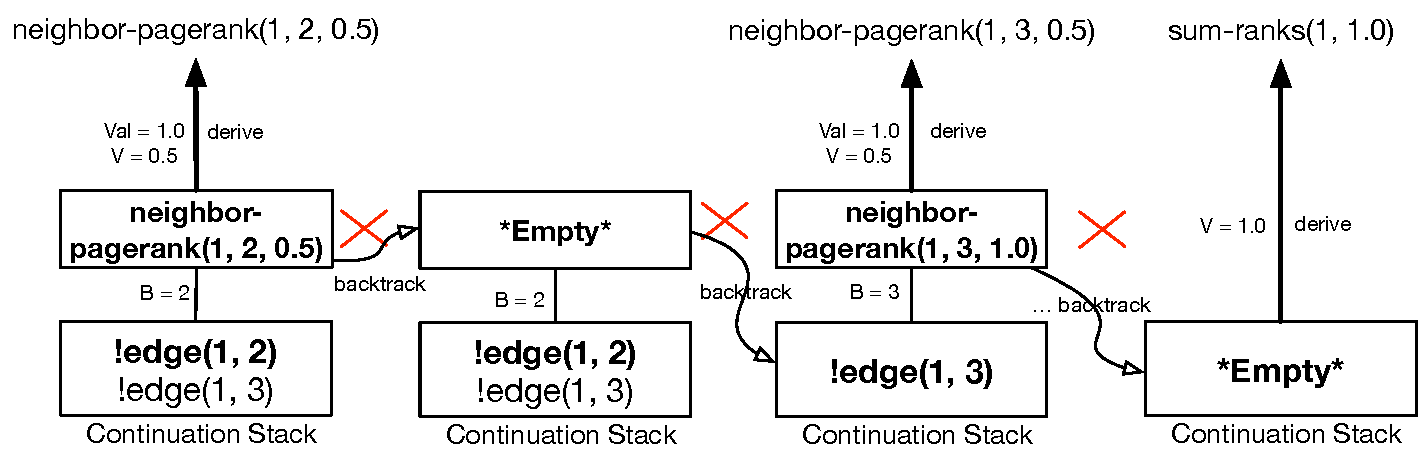
\includegraphics[width=0.85\linewidth]{figures/logical_foundations/backtrack.pdf}
   \end{center}
   \caption{Generating the PageRank aggregate.}
   \label{fig:logic:backtrack}
\end{figure}

\subsubsection{Matching}

The matching state for aggregates is 
$\matstatea{\Delta_N}{\lstack{C};
   \lstack{P}}{\Gamma}{\Delta}{\Omega}{\Delta' \rightarrow \Omega'}{\Sigma}$

\begin{enumerate}
   \item[$\Omega_N$] ordered list of remaining terms of the head of the rule to
   be derived;

   \item[$\Delta_N$] multi-set of linear facts that were still available after
   matching the body of the rule and all the previous aggregates. Note that
   $\Delta, \Xi = \Delta_N$;

   \item[$\Xi$] multi-set of linear facts used during the matching process of
   the body of the rule and all the previous aggregates;

   \item[$\Gamma_{1}$] set of persistent facts derived up to this point in the
   head of the rule;

   \item[$\Delta_{1}$] multi-set of linear facts derived up to this point in
   the head of the rule;

   \item[$\Delta'$] multi-set of linear facts consumed up to this point;

   \item[$\Omega'$] terms matched using $\Delta'$ up to this point;

   \item[$\m{agg}$] aggregate that is being matched;

   \item[$\Sigma$] the list of aggregated values;

   \item[$\lstack{C}$] continuation stack that contains both linear and persistent
   frames. The first frame must be linear;

   \item[$\lstack{P}$] initial part of the continuation stack with only persistent
   frames;

   \item[$\Delta$] multi-set of linear facts remaining up to this point in the
   matching process;

   \item[$\Omega$] ordered list of terms that need to be matched for the
   comprehension to be applied.

\end{enumerate}

Since aggregates accumulate values (from specific variables), we retrieved the
value from the $\Psi$ context. Remember that $\Psi$ is used for the
quantification connectives in the sequent calculus and in LLD is used to store
current variable bindings.

\subsubsection{Linear fact expressions}

The following two transitions deal with the case when there is a linear
fact expression in the body of the aggregate.


\begin{multline}
\transx{
   \matstatea{\deltan}{\lstack{C};
      \lstack{P}}{\Gamma}{\Delta, p_1, \Delta''}{p, \Omega}{\Delta' \rightarrow
         \Omega'}{\Sigma}
}
{
   \matstatea{\deltan}{\lframe{\Delta,
   p_1}{\Delta''}{p}{\Omega}{\Delta'}{\Omega'}, \lstack{C}; \lstack{P}}{\Gamma}{\Delta,
      \Delta''}{\Omega}{\Delta', p \rightarrow \Omega' \otimes
      p}{\Sigma}\tag{agg match p ok}
}
\end{multline}

\[
\trans{
   \matstatea{\deltan}{\lstack{C}; \lstack{P}}{\Gamma}{\Delta}{p,
      \Omega}{\Delta' \rightarrow \Omega'}{\Sigma}
}
{
   \contstatea{\deltan}{\lstack{C} ; \lstack{P}}{\Gamma}{\Sigma}
}\tag{agg match p fail}
\]


\subsubsection{Persistent fact expressions}

The transitions for dealing with persistent facts are similar to the previous
ones.



\[
\trans{
   \matstatea{\Delta_N}{\cdot;
      \lstack{P}}{\Gamma, p_1, \Gamma''}{\Delta}{\bang p, \Omega}{\Delta' \rightarrow
         \Omega'}{\Sigma}
}
{
   \matstatea{\Delta_N}{\cdot; \pframe{\Gamma''}{\Delta}{\bang
   p}{\Omega}{\Delta'}{\Omega'}, \lstack{P}}{\Gamma, p_1, \Gamma''}{\Delta}{\Omega}
   {\Delta' \rightarrow \Omega' \otimes \bang p}{\Sigma}
}
\]

\[
\trans{
   \matstatea{\Delta_N}{\lstack{C};
      \lstack{P}}{\Gamma, p_1, \Gamma''}{\Delta}{\bang p, \Omega}{\Delta' \rightarrow
         \Omega'}{\Sigma}
}
{
   \matstatea{\Delta_N}{\pframe{\Gamma''}{\Delta}{\bang
   p}{\Omega}{\Delta'}{\Omega'}, \lstack{C} ; \lstack{P}}{\Gamma, p_1, \Gamma''}{\Delta}{\Omega}
   {\Delta' \rightarrow \Omega' \otimes \bang p}{\Sigma}
}
\]


\[
\trans{
   \matstatea{\Delta_N}{\lstack{C}; \lstack{P}}{\Gamma}{\Delta}{\bang p,
      \Omega}{\Delta' \rightarrow \Omega'}{\Sigma}
}
{
   \contstatea{\Delta_N}{\lstack{C} ; \lstack{P}}{\Gamma}{\Sigma}
}
\]



\subsubsection{Deconstruct body}


\begin{multline}
\transx{
   \matstatea{\deltan}{\lstack{C};
      \lstack{P}}{\Gamma}{\Delta}{X \otimes Y, \Omega}{\Delta' \rightarrow
         \Omega'}{\Sigma}
}
{
   \matstatea{\deltan}{\lstack{C};
      \lstack{P}}{\Gamma}{\Delta}{X, Y, \Omega}{\Delta' \rightarrow
         \Omega'}{\Sigma}
} \tag{agg match $\otimes$}
\end{multline}

\begin{multline}
\transx{
   \matstatea{\deltan}{\lstack{C};
      \lstack{P}}{\Gamma}{\Delta}{\one, \Omega}{\Delta' \rightarrow
         \Omega'}{\Sigma}
}
{
   \matstatea{\deltan}{\lstack{C};
      \lstack{P}}{\Gamma}{\Delta}{\Omega}{\Delta' \rightarrow
         \Omega'}{\Sigma}
      } \tag{agg match $\one$}
\end{multline}



\subsubsection{Successful match}

When the aggregate body finally matches, we retrieve the term for variable $x$
(the aggregate variable) and add it to the list $\Sigma$.

\[
\infer[\ma{AG} \m{end}]
{\ma{AG} \Psi; \Gamma; \Delta; \Xi_N; \Gamma_{N1}; \Delta_{N1}; \Xi; \cdot;
   \lstack{C}; \lstack{P}; \Omega_N; \Delta_N; \Sigma \rightarrow \outsem}
{\fixa{AG} \Gamma; \Xi_N; \Gamma_{N1}; \Delta_{N1}; \Xi; \lstack{C}; \lstack{P}; \Omega_N;
   \Delta_N; V :: \Sigma \rightarrow \outsem & x : V : \tau \in \Psi}
\]


\subsubsection{Continuation stack update}

As we said before, to update the continuation stacks, we need remove to all the
frames except the first linear frame and remove the consumed linear facts from
the remaining frames so that they are still valid for the next application of
the aggregate.  The judgment that updates the stack has the form
$\fixstatea{\Delta}{\Xi; \Delta'}{\lstack{C};
   \lstack{P}}{\Gamma}{\Sigma}$, where:

\begin{enumerate}
   \item[$\Omega_N$] ordered list of remaining terms of the head of the rule to
   be derived;
   \item[$\Delta$] multi-set of linear facts that were still available after
   matching the body of the rule and the body of the aggregate;
   \item[$\Xi$] multi-set of linear facts used during the matching process of
   the body of the rule and all the previous aggregates;
   \item[$\Delta'$] multi-set of linear facts consumed by the aggregate body;
   \item[$\Gamma_{1}$] set of persistent facts derived by the head of the rule
   and all the previous aggregates;
   \item[$\Delta_{1}$] multi-set of linear facts derived by the head of the
   rule and all the previous aggregates;
   \item[$\m{agg}$] the current aggregate;
   \item[$\Sigma$] list of accumulated values;
   \item[$\lstack{C}, \lstack{P}$] continuation stacks for the comprehension;
   \item[$\Gamma$] set of usable persistent facts.
\end{enumerate}

\subsubsection{Remove linear continuation frames}

To remove all linear continuation frames except the first one, we simply go
through all the frames in the stack $\lstack{C}$ until only one frame remains.
This last frame and stack $\lstack{P}$ are then updated by removing $\Delta'$
from its contexts.


{\tiny
\[
\infer[\fixa ~\m{end~linear}]
{\fixa \Gamma; \Xi_N; \Gamma_{N1}; \Delta_{N1}; \Xi; (\Delta_x; \Delta''; \cdot;
      p; \Omega; \cdot; \Upsilon); P;  \aggsz{A}{B}{C}; \Omega_N; \Delta_N; T \rightarrow \Xi'; \Delta'; \Gamma'}
{\begin{split}\strans &\Xi; P; P' \\ \da \Gamma; \Xi_N, \Xi; \Gamma_{N1};
   \Delta_{N1}; B; (\Delta_x - \Xi; \Delta'' - \Xi; \cdot;& p; \Omega; \cdot;
         \Upsilon) ; P' ; \aggsz{A}{B}{C}; \Omega_N; (\Delta_N - \Xi); T &\rightarrow \Xi'; \Delta'; \Gamma'\end{split}}
\]
}

\[
\infer[\fixa \m{more}]
{\fixa \Gamma; \Xi_N; \Gamma_{N1}; \Delta_{N1}; \Xi; \_, X, C; P; AG; \Omega_N; \Delta_N; T \rightarrow \Xi'; \Delta'; \Gamma'}
{\fixa \Gamma; \Xi_N; \Gamma_{N1}; \Delta_{N1}; \Xi; X, C; P; AG; \Omega_N; \Delta_N; T \rightarrow \Xi'; \Delta'; \Gamma'}
\]

{\footnotesize
\[
\infer[\fixa \m{end~empty}]
{\fixa \Gamma; \Xi_N; \Gamma_{N1}; \Delta_{N1}; \Xi; \cdot; P; \aggsz{A}{B}{C}; \Omega_N; \Delta_N; T \rightarrow \Xi'; \Delta'; \Gamma'}
{\begin{split}\strans &\Xi; P; P' \\ \da \Gamma; \Xi_N, \Xi; \Gamma_{N1};
   \Delta_{N1}; B; \cdot ; P' ; &\aggsz{A}{B}{C}; \Omega_N; (\Delta_N - \Xi); T &\rightarrow \Xi'; \Delta'; \Gamma'\end{split}}
\]
}


\subsubsection{Aggregate backtracking}

If the aggregate match fails, we need to backtrack to the next candidate fact.
The backtracking state 
has the form
$\contstatea{\Delta_N}{\lstack{C} ; \lstack{P}}{\Gamma}{\Sigma}$, where:

\begin{enumerate}
   \item[$\Omega_N$] ordered list of remaining terms of the head of the rule to
   be derived;
   \item[$\Delta_N$] multi-set of linear facts that were still available after
   matching the body of the rule and the body of the aggregate;
   \item[$\Xi$] multi-set of linear facts used during the matching process of
   the body of the rule and all the previous aggregates;
   \item[$\Gamma_{1}$] set of persistent facts derived by the head of the rule
   and all the previous aggregates;
   \item[$\Delta_{1}$] multi-set of linear facts derived by the head of the
   rule and all the previous aggregates;
   \item[$\m{agg}$] the current aggregate;
   \item[$\Sigma$] list of accumulated values.
   \item[$\lstack{C}, \lstack{P}$] continuation stacks for the comprehension;
   \item[$\Gamma$] set of usable persistent facts.
\end{enumerate}

\paragraph{Using the $\lstack{C}$ stack}

The following 4 state transitions use the $\lstack{C}$ stack, the stack where the
first continuation frame is linear, to perform backtracking.


\begin{multline}
\transx{
   \contstatea{\deltan}{\lframe{\Delta}{p_1, \Delta''}{p}{\Omega}{\Delta'}{\Omega'}, \lstack{C} ; \lstack{P}}{\Gamma}{\Sigma}
}
{
   \matstatea{\deltan}{\lframe{\Delta,
      p_1}{\Delta''}{p}{\Omega}{\Delta'}{\Omega'}, \lstack{C}; \lstack{P}}{\Gamma}{\Delta}{p,
      \Omega}{\Delta', p_1 \rightarrow \Omega' \otimes p}{\Sigma}
} \tag{agg next p $\lstack{C}$}
\end{multline}

\begin{multline}
\transx{
   \contstatea{\deltan}{\pframe{p_1, \Gamma''}{\Delta}{\bang
   p}{\Omega}{\Delta'}{\Omega'}, \lstack{C} ; \lstack{P}}{\Gamma}{\Sigma}
}
{
   \matstatea{\deltan}{\pframe{\Gamma''}{\Delta}{\bang p}
      {\Omega}{\Delta'}{\Omega'}, \lstack{C}; \lstack{P}}{\Gamma}{\Delta}{p,
      \Omega}{\Delta' \rightarrow \Omega' \otimes \bang p}{\Sigma}
} \tag{agg next \bang p $\lstack{C}$}
\end{multline}

\[
\trans{
   \contstatea{\deltan}{\lframe{\Delta}{\cdot}{p}{\Omega}{\Delta'}{\Omega'}, \lstack{C} ; \lstack{P}}{\Gamma}{\Sigma}
}
{
   \contstatea{\deltan}{\lstack{C} ; \lstack{P}}{\Gamma}{\Sigma}
} \tag{agg  next frame $\lstack{C}$}
\]

\[
\trans{
   \contstatea{\deltan}{\pframe{\cdot}{\Delta}{\bang
   p}{\Omega}{\Delta'}{\Omega'}, \lstack{C} ; \lstack{P}}{\Gamma}{\Sigma}
}
{
   \contstatea{\deltan}{\lstack{C} ; \lstack{P}}{\Gamma}{\Sigma}
} \tag{agg next \bang frame $\lstack{C}$}
\]


\paragraph{Using the $\lstack{P}$ stack}

The following 2 state transitions rules use the $\lstack{P}$ stack instead, the stack where all
continuation frames are persistent.

\[
\infer[\conta{AG} \m{next}~\lstack{P}~\bang p]
{\conta{AG} \Gamma; \Delta_N; \Xi_N; \Gamma_{N1}; \Delta_{N1}; \cdot; f, \lstack{P}; \Omega_N; \Sigma \rightarrow \outsem}
{\begin{gathered}
   f = [p_1, \Gamma'; \Delta_N; \cdot; \bang p; \Omega; \cdot; \Upsilon] \\
   f' = [\Gamma'; \Delta_N; \cdot; \bang p; \Omega; \cdot; \Upsilon] \\
   \ma{AG} \Gamma; \Delta_N; \Xi_N; \Gamma_{N1}; \Delta_{N1}; \cdot; \Omega; \cdot;
      f', \lstack{P}; \Omega_N; \Delta_N; \Sigma \rightarrow \outsem
 \end{gathered}
}
\]

\[
\infer[\conta{AG} \m{next}~\lstack{P}~\m{empty}~\bang p]
{\conta{AG} \Gamma; \Delta_N; \Xi_N; \Gamma_{N1}; \Delta_{N1}; \cdot; f, \lstack{P}; \Omega_N; \Sigma
   \rightarrow \outsem}
{\begin{gathered}
   f =  [\cdot; \Delta_N; \cdot; \bang p; \Omega; \cdot; \Upsilon] \\
   \conta{AG} \Gamma; \Delta_N; \Xi_N; \Gamma_{N1}; \Delta_{N1}; \cdot; \lstack{P};
      \Omega_N; \Sigma \rightarrow \outsem
 \end{gathered}
}
\]


\paragraph{Aggregate done}

If both the $\lstack{C}$ and $\lstack{P}$ stacks are empty, backtracking is
impossible and the aggregate is done. The final head of the aggregate is then
derived along with the rest of the rule's head.

\[
\infer[\conta{\aggsz{A}{B}{C}} \m{end}]
{\conta{\aggsz{A}{B}{C}} \Gamma; \Delta_N; \Xi_N; \Gamma_{N1}; \Delta_{N1}; \cdot; \cdot;
   \Omega; \Sigma \rightarrow \outsem}
{\done \Gamma; \Delta_N; \Xi_N; \Gamma_{N1}; \Delta_{N1}; (\lambda x. C
      x)\Sigma,
   \Omega \rightarrow \outsem}
\]


\subsubsection{Aggregate Derivation}

After updating the continuation stacks, the subhead of the aggregate is derived.
The derivation state has the form
$\derstatea{\Delta}{\Xi}{\Gamma_1}{\Delta_1}{\Sigma}{\lstack{C};
   \lstack{P}}{\Omega}$, where:

\begin{enumerate}
   \item[$\Omega_N$] ordered list of remaining terms of the head of the rule to
   be derived;
   \item[$\Delta$] multi-set of remaining linear facts that can be used for
   the next aggregate applications.
   \item[$\Xi$] multi-set of linear facts consumed both by the body of the rule
   and previous aggregate applications;
   \item[$\Gamma_1$] set of persistent facts derived by the head of the rule,
   previous aggregates and current derivation;
   \item[$\Delta_1$] multi-set of linear facts derived by the head of the rule,
   previous aggregates and current derivation;
   \item[$\m{agg}$] current aggregate symbol;
   \item[$\Sigma$] accumulated list of values of the aggregate;
   \item[$\lstack{C}, \lstack{P}$] new continuation stacks;
   \item[$\Gamma$] set of persistent facts;
   \item[$\Omega$] ordered list of terms to derive.
\end{enumerate}

\[
\infer[\da{AG} p]
{\da{AG} \Gamma; \Delta_N; \Xi_N; \Gamma_1; \Delta_1; p, \Omega; \lstack{C}; \lstack{P}; \Omega_N;
   \Sigma \rightarrow \outsem}
{\da{AG} \Gamma; \Delta_N; \Xi_N; \Gamma_1; \Delta_1, p; \Omega; \lstack{C}; \lstack{P}; \Omega_N;
   \Sigma \rightarrow \outsem}
\]

\[
\infer[\da{AG} \bang p]
{\da{AG} \Gamma; \Delta_N; \Xi_N; \Gamma_1; \Delta_1; \bang p, \Omega; \lstack{C};
   \lstack{P}; \Omega_N; \Sigma \rightarrow \outsem}
{\da{AG} \Gamma; \Delta_N; \Xi_N; \Gamma_1, p; \Delta_1; \Omega; \lstack{C}; \lstack{P}; \Omega_N;
   \Sigma \rightarrow \outsem}
\]

\[
\infer[\da{AG} \otimes]
{\da{AG} \Gamma; \Delta_N; \Xi_N; \Gamma_1; \Delta_1; A \otimes B, \Omega; \lstack{C}; \lstack{P}; \Omega_N;
   \Sigma \rightarrow \outsem}
{\da{AG} \Gamma; \Delta_N; \Xi_N; \Gamma_1; \Delta_1; A, B, \Omega; \lstack{C}; \lstack{P}; \Omega_N;
   \Sigma \rightarrow \outsem}
\]

\[
\infer[\da{AG} \m{end}]
{\da{AG} \Gamma; \Delta_N; \Xi_N; \Gamma_1; \Delta_1; \cdot; \lstack{C}; \lstack{P}; \Omega_N;
   \Sigma \rightarrow \outsem}
{\conta{AG} \Gamma; \Delta_N; \Xi_N; \Gamma_1; \Delta_1; \lstack{C}; \lstack{P}; \Omega_N; \Sigma
   \rightarrow \outsem}
\]



This completes the specification of LLD.



